% ---------------------------------------------------------
% Estilo, Pacotes e Defini��es Pr�vias
% ---------------------------------------------------------

\documentclass[tese]{tese_eesc}
\usepackage[brazilian]{babel}
\usepackage[T1]{fontenc}
\usepackage[latin1]{inputenc}
\usepackage{natbib} 
%mathpazo % Muda a fonte para Palatino
\usepackage{array,rotating,setspace,enumerate} 
\usepackage{float,amssymb,amstext}
\usepackage[cmex10]{amsmath}
\usepackage{booktabs,multirow,dcolumn}
\usepackage{pstricks,pst-node,pst-coil,pst-plot,pst-tree}
\usepackage{subfig,remreset}
\usepackage{graphicx}
\usepackage{epstopdf}

%%%%%%%%%%%%%%%%%%%%%%%%%%%%%%%%%%%%%%%%%%%%
%%%%% Algoritmo para encapsular c�digo %%%%% 
\usepackage{listings}
\usepackage{color}
 
\definecolor{dkgreen}{rgb}{0,0.5,0}
\definecolor{gray}{rgb}{0.5,0.5,0.5}
\definecolor{mauve}{rgb}{0.58,0,0.82}
 
\lstset{
  language=bash,                
  basicstyle=\footnotesize,           
  numbers=left,                   
  numberstyle=\tiny\color{gray},  
  stepnumber=1,                             
  numbersep=5pt,                  
  backgroundcolor=\color{white},    
  showspaces=false,               
  showstringspaces=false,         
  showtabs=false,                 
  frame=single,                   
  rulecolor=\color{black},        
  tabsize=2,                      
  captionpos=,                   
  breaklines=true,                
  breakatwhitespace=false,        
  title=\lstname,                               
  keywordstyle=\color{blue},          
  commentstyle=\color{dkgreen},       
  stringstyle=\color{mauve},     
}

%%%%%%%%%%%%%%%%%%%%%%%%%%%%%%%%%%%%%%%%%%%%%

\renewcommand{\sin}{\text{sen}}

\newcommand{\xdi}{x_{d_i}}
\newcommand{\xqi}{x_{q_i}}
\newcommand{\xldi}{x^\prime_{d_i}}
\newcommand{\xlqi}{x^\prime_{q_i}}
\newcommand{\eldi}{E^\prime_{d_i}}
\newcommand{\elqi}{E^\prime_{q_i}}
\newcommand{\efdi}{E_{fd_i}}
\newcommand{\idi}{I_{d_i}}
\newcommand{\iqi}{I_{q_i}}
\newcommand{\vi}[1]{V^{#1}_i}
\newcommand{\vk}[1]{V^{#1}_k}
\newcommand{\ti}[1]{\theta^{#1}_i}
\newcommand{\tk}[1]{\theta^{#1}_k}
\newcommand{\ii}[1]{I^{#1}_i}
\newcommand{\iir}[1]{I^{#1}_{i_\text{re}}}
\newcommand{\iii}[1]{I^{#1}_{i_\text{im}}}
\newcommand{\ri}[1]{R^{#1}_i}
\newcommand{\rsi}[1]{R_{#1_i}}
\newcommand{\xxi}[1]{X^{#1}_i}
\newcommand{\pli}[1]{P^{#1}_{L_i} \left( \vi{#1} \right)}
\newcommand{\qli}[1]{Q^{#1}_{L_i} \left( \vi{#1} \right)}
\newcommand{\ybgik}{Y^{\beta\gamma}_{ik}}
\renewcommand{\exp}[1]{\text{e}^{j#1}}
\newcommand{\vicos}[1]{\vi{#1}\cos\ti{#1}}
\newcommand{\vicosp}[2]{\vi{#1}\cos\left(\ti{#1} #2 2\pi/3\right)}
\newcommand{\visin}[1]{\vi{#1}\sin\ti{#1}}
\newcommand{\visinp}[2]{\vi{#1}\sin\left(\ti{#1} #2 2\pi/3\right)}
\newcommand{\cosp}{\cos \left( 2\pi / 3 \right)}
\newcommand{\sinp}{\sin \left( 2\pi / 3 \right)}
\newcommand{\tni}[1]{T_{n#1_i}}
\newcommand{\tdi}[1]{T_{d#1_i}}
\newcommand{\twi}{T_{w_i}}
\newcommand{\xci}[1]{x_{#1_i}^c}
\newcommand{\xgi}[1]{x_{#1_i}^g}
\newcommand{\derp}[2]{\frac{\partial #1}{\partial #2}}
\newcommand{\pder}[2]{\frac{\partial #1}{\partial #2}}
\newcommand{\ft}{\left( t \right)}

\newcommand{\vicosder}[1]{\cos\tio{#1}\Delta\vi{#1}-\vio{#1}\sin\tio{#1}\Delta\ti{#1}}
\newcommand{\visinder}[1]{\sin\tio{#1}\Delta\vi{#1}+\vio{#1}\cos\tio{#1}\Delta\ti{#1}}
\newcommand{\vicospder}[2]{\cos\left(\tio{#1} #2 2\pi/3\right)\Delta\vi{#1} - \vio{#1}\sin\left(\tio{#1} #2 2\pi/3\right)\Delta\ti{#1}}
\newcommand{\visinpder}[2]{\sin\left(\tio{#1} #2 2\pi/3\right)\Delta\vi{#1} + \vio{#1}\cos\left(\tio{#1} #2 2\pi/3\right)\Delta\ti{#1}}

\newcommand{\eldio}{E^\prime_{d_{i_\text{e}}}}
\newcommand{\elqio}{E^\prime_{q_{i_\text{e}}}}
\newcommand{\vio}[1]{V^{#1}_{i_\text{e}}}
\newcommand{\vko}[1]{V^{#1}_{k_\text{e}}}
\newcommand{\tio}[1]{\theta^{#1}_{i_\text{e}}}
\newcommand{\tko}[1]{\theta^{#1}_{k_\text{e}}}
\newcommand{\iio}[1]{I^{#1}_{i_\text{e}}}
\newcommand{\iiro}[1]{I^{#1}_{i_{\text{re}_\text{e}}}}
\newcommand{\iiio}[1]{I^{#1}_{i_{\text{im}_\text{e}}}}
\newcommand{\idio}{I_{d_{i_\text{e}}}}
\newcommand{\iqio}{I_{q_{i_\text{e}}}}

\newcolumntype{.}{D{.}{.}{-1}}

\renewcommand{\labelitemi}{\tiny$\blacksquare$\normalsize}


\makeatletter
\@removefromreset{footnote}{chapter}
\makeatother


% ---------------------------------------------------------
% Informa��es da Tese (T�tulo, Nomes, Palavras-chave, ...)
% ---------------------------------------------------------

% ------------------------------------------
% T�tulo
% ------------------------------------------
\title{Plataforma para aplica��es de Tempo-Real usando Linux embarcado em microcontroladores ARM}
% ------------------------------------------
% Autor, Departamento, Data
% ------------------------------------------
\author{Soares Passos}{Leonardo Br�s}
\depmt{Departamento de Engenharia El�trica}
\course{Engenharia El�trica - �nfase em Sistemas de Energia e Automa��o}
\date{Novembro}{2012}{26}

% ------------------------------------------
% Orientador e Banca
% ------------------------------------------
\advisor[Prof.~Dr.]{Rodrigues}{Evandro Lu�s L.}
\advisorwidth{9.7cm}
\advisorinfo{Universidade de S�o Paulo -- Escola de Engenharia de S�o Carlos}{Doutor pela Universidade de S�o Paulo -- S�o Carlos, Brasil}
\examiner[Prof.~Dr.]{Monteiro}{Jos� Roberto Boffino de Almeida}
\examinerinfo{Universidade de S�o Paulo -- Escola de Engenharia de S�o Carlos}{Doutor pela Universidade de S�o Paulo -- S�o Carlos, Brasil}
\examiner[Doutorando]{Monaro}{Renato Machado}
\examinerinfo{Universidade de S�o Paulo -- Escola de Engenharia de S�o Carlos}{Doutorando pela Universidade de S�o Paulo -- S�o Carlos, Brasil}

% ------------------------------------------
% Palavras-chave
% ------------------------------------------
\keyword{Automa��o}
\keyword{Microcontroladores}
\keyword{Linux}
\keyword{ARM}
\keyword{Real Time}
\keyword{embarcado}
\keyword{Software Livre}



% ---------------------------------------------------------------
% Elementos Pr�-textuais e Listas de Figuras, Tabelas, e Sum�rio
% ---------------------------------------------------------------

\begin{document}
\maketitle

% ---------------------------------------
% Ep�grafe
% ---------------------------------------

\epigrafe {Imagina��o � mais importante que o conhecimento. Conhecimento � limitado, enquanto a imagina��o envolve todo o mundo, estimulando o progresso, dando vida � evolu��o. Ela �, de maneira rigorosa, um fator real na pesquisa cient�fica.}{Albert Eninstein, 1931}

% ---------------------------------------
% Dedicat�ria
% ---------------------------------------

\dedicatoria{� minha fam�lia,\\ que sempre me apoiou nos momentos dif�ceis.}


% ---------------------------------------
% Agradecimentos
% ---------------------------------------

\begin{agradecimentos}

� minha m�e, Maria Aparecida, que me apoiou durante toda minha vida, e me ensinou a perseguir meus sonhos atrav�s de esfor�o e dedica��o.

Ao meu pai, Juvenal Milton, que me ensinou a import�ncia de aplicar meus conhecimentos de maneira pr�tica.

� L�gia, minha irm�, que sempre me ensinou a n�o me contentar com meias vit�rias e a continuamente buscar a melhoria.

� Giselle e ao Marcos, minha irm� e seu marido, que me ensinaram a import�ncia da boa manuten��o dos relacionamentos pessoais.

� Aline, minha irm�, que apesar dessa �poca de desentendimento, sempre me encorajou a manter um pensamento cr�tico.

Aos meus av�s, pois cada um deles teve grande colabora��o no meu crescimento pessoal. 

Ao Prof. Evandro, que me orientou, aconselhou e animou nos momentos mais complicados da gradua��o.

Aos amigos que conheci durante a gradua��o, com quem aprendi a apreciar as diferen�as entre as pessoas.

Aos professores do departamento, que me ensinaram preciosas li��es, mesmo que, por vezes, da maneira dif�cil.

� Universidade de S�o Paulo, que me aceitou como aluno e disponibilizou recursos para minha gradua��o.

Aos cidad�os brasileiros, que pagam seus impostos e contribuem para a manuten��o de universidades p�blicas, gratuitas e de qualidade.

\end{agradecimentos}


% ---------------------------------------
% Resumo e Abstract
% ---------------------------------------

\begin{abstract} 

Devido �s crescentes necessidades de automa��o e controle de sistemas de tempo-real, que t�m rigorosos requisitos de previsibilidade do tempo de resposta, mostra-se vi�vel a utiliza��o de Sistemas Operacionais de tempo-real embarcados, cujo objetivo �, al�m de atender os requisitos impostos, simplificar e acelerar o desenvolvimento do software de controle. 
Nesse trabalho, usou-se o Linux, juntamente com o \textit{patch RT}, tamb�m de c�digo aberto, para construir um Sistema Operacional de Tempo-Real para a arquitetura ARM, o qual foi carregado no Kit de Desenvolvimento SAM9-L9260. 
Foram ent�o realizados testes de desempenho, cuja fun��o foi medir o tempo de resposta do conjunto. A partir de tais testes, usando-se de compara��o com o Linux sem a aplica��o do \textit{patch}, constatou-se expressiva melhora de desempenho do sistema operacional em rela��o �s tarefas de tempo-real, demonstrando elevada aplicabilidade e reduzido custo de implementa��o, tornando economicamente vi�veis novas aplica��es RT em automa��o.

\end{abstract}

\begin{englishabstract}{Automation, Microcontrollers, MCU, Linux, ARM, Real-Time, Embedded, Open Source}

Due to the growing needs of automation and control of real-time systems, which have strict requirements of response time predictability, it is shown viable the use of embedded real-time operating systems, whose goal is, in addition to meeting the imposed requirements, simplify and accelerate the development of the control software.
In this final thesis, it was used Linux, along with the \textit{RT patch}, also open source, to build a Real-Time operating system targeted to ARM architecture, which was loaded on a SAM9-L9260 Development Kit. 
So, there were conducted performance tests, whose function were measuring the response time of this ensemble. From these tests, using comparison with Linux without implementation of the patch, it was observed great improvement on Linux performance in regard to real-time tasks, demonstrating high applicability and reduced implementation cost, making economically viable new RT automation applications.

\end{englishabstract}


% --------------------------------------------------------------
% Listas de Figuras, Tabelas, Abreviaturas, S�mbolos e Sum�rio
% --------------------------------------------------------------

\listoffigures
\listoftables

\begin{listofabbrv}{ESPRIT~}
	\item[OS] Sistema Operacional -- \textit{Operating System}
	\item[RT] Tempo Real -- \textit{Real Time}
	\item[RTS] Sistema de Tempo Real -- \textit{Real Time System}
	\item[RTOS] Sistema Operacional de Tempo Real -- \textit{Real Time Operating System}
	\item[FOSS] Software Livre e de C�digo Aberto -- \textit{Free Open Source Software}
	\item[MCU] Microcontrolador -- \textit{Microcontroller Unit}
	\item[CPU] Microprocessador -- \textit{Central Processing Unit}
	\item[ARM] M�quinas RISC Avan�adas -- Advanced RISC Machines
	\item[RISC] Conjunto de Comandos Reduzido -- \textit{Reduced Intruction Set Computing}
	\item[CISC] Conjunto de Comandos Complexo -- \textit{Complex Intruction Set Computing}
	\item[RootFS] Parti��o Raiz do Sistema Operacional -- \textit{Root File System}
	\item[USB] Barramento Serial Universal -- \textit{Universal Serial Bus}
	\item[GPIO] Pino de Entrada e Sa�da Gen�rico -- \textit{General Pourpose Input Oputput}
	\item[APT] Ferramenta de Empacotamento Avan�ada -- \textit{Advanced Packaging Tool} 
	\item[SSH] Terminal de Acesso Remoto Seguro -- \textit{Secure Shell}
	\item[PIC] Controlador de Interface Program�vel -- \textit{Programmable Interface Controller}

\end{listofabbrv}
											% REVISADO
\tableofcontents


% ---------------------------------------------------------
% Corpo do trabalho (capitulos)
% ---------------------------------------------------------

\chapter{Introdu��o}
\label{cap:intro}


Nas duas �ltimas d�cadas, a utiliza��o de Microcontroladores para Automa��o de Processos se tornou muito popular por sua elevada efici�ncia e custo reduzido. 
Dentre os microcontroladores mais simples, como o 8051 e alguns PICs (\textit{Programmable Interface Controller}), � comum desenvolver as funcionalidades da aplica��o usando linguagem C, ou, �s vezes, simplesmente linguagem \textit{Assembly}. Gra�as ao uso dessas linguagens de baixo n�vel � poss�vel ter uma eficiente previsibilidade dos tempos de execu��o das aplica��es desenvolvidas.

Ao longo dos anos, em busca de ganhos elevados de velocidade e efici�ncia, os microcontroladores vem sofrendo modifica��es que se inclinam para aumento de Conjunto de Comandos, Espa�o de Endere�amento e Frequ�ncia de opera��o, al�m de modifica��es que incluem novos recursos mais avan�ados. 
Algumas dessas modifica��es, entretanto, tornam a programa��o do microcontrolador mais complexa, resultando na inviabilidade do uso de linguagens de baixo n�vel para sua programa��o.

Para auxiliar na solu��o do problema da complexidade, utiliza-se cada vez mais Sistemas Operacionais (SO) reduzidos, que ficam respons�veis por administrar os recursos da plataforma, e sobre os quais � realizado o desenvolvimento da aplica��o desejada. 
No contexto geral, esse conceito trouxe grandes melhorias, inclusive no tempo de desenvolvimento [\cite{osT}]. No entanto, uma vez que os tempos e recursos do sistema n�o ficam mais sob controle do desenvolvedor, n�o h� como garantir a previsibilidade dos tempos de execu��o das aplica��es.

Para suprir a necessidade de algumas aplica��es que precisam de previsibilidade de resposta (chamadas aplica��es de Tempo Real) [\cite{RTbook}], foram propostos os Sistemas Operacionais de Tempo Real (RTOS), que, para determinadas tarefas, tem a fun��o de garantir que o sistema responda com um tempo previs�vel, e quando poss�vel, reduzido.

Anteriormente, al�m do custo elevado de Microcontroladores de alto desempenho, os RTOS, que funcionavam sobre estes, constitu�am-se principalmente de softwares propriet�rios, fechados e com alto custo de aquisi��o, o que limitava o uso dessas plataformas �s grandes corpora��es.
Hoje, com a incr�vel redu��o de pre�os dos microcontroladores de alto desempenho, e o surgimento de algumas alternativas de RTOS em Software Livre, fez-se poss�vel a explora��o desses recursos para projetos de baixo custo.
 
A r�pida evolu��o dos Microcontroladores nos �ltimos anos acontece tamb�m devido ao crescente mercado de \textit{Smartphones} e \textit{Tablets}. Esse mercado busca, cada vez mais, elevar o poder de processamento, reduzir a pot�ncia consumida e reduzir o custo de seus dispositivos. 
Assim, tal mercado optou por adotar, em sua maioria, o uso da arquitetura de microcontroladores ARM (\textit{Advanced RISC Machines}) para seus produtos, e por isso o pre�o e a disponibilidade desses microcontroladores os tornaram interessantes para o desenvolvimento de projetos mais simples.

Al�m disso, o pr�prio mercado de \textit{Tablets} e \textit{Smartphones}, visando reduzir seu custo, tem investido bastante no desenvolvimento de software livre, sendo o Linux o maior beneficiado: 
mais de 64\% dos Celulares vendidos no segundo trimestre de 2012 carregam o Android [\cite{MobileStat}], o SO do Google que utiliza kernel Linux, sendo que este, atualmente, � o mais bem sucedido projeto de SO Livre. Devido ao fato de seu c�digo fonte ser aberto ao p�blico e possuir uma boa documenta��o, h� muita facilidade em adapt�-lo a necessidades particulares.

Nesse contexto, unindo a disponibilidade de microcontroladores com o crescente desenvolvimento do software livre, � vi�vel a utiliza��o do Linux em Sistemas Embarcados para realiza��o de automa��o e controle de sistemas, incluindo os de tempo real.


\section{Objetivos} 

Tendo em vista o cen�rio atual para desenvolvimento em plataformas embarcadas, o principal objetivo deste trabalho � desenvolver uma Plataforma de Automa��o com as seguintes caracter�sticas:

\begin{itemize}
\item Caracterize-se por um baixo custo de implementa��o;
\item Tenha embarcado o sistema operacional Linux, com uma distribui��o est�vel;
\item Funcione a partir de um microcontrolador ARM de bom desempenho e baixo custo;
\item Seja control�vel via internet, atrav�s de uma interface Web;
\item Ofere�a uma segura previsibilidade de tempos de execu��o, ou seja, comporte-se como um RTOS;
\item Seja altamente personaliz�vel.

\end{itemize}


\section{Justificativa}

O desenvolvimento de uma plataforma de automa��o de baixo custo, que usufrua de RTOS deve possibilitar a oportunidade de desenvolvimento de aplica��es para automa��o, de forma geral, hoje ainda pouco exploradas com esse conceito.


\section{Organiza��o do Trabalho}
Este trabalho est� estruturado por cap�tulos, sendo eles divididos da seguinte maneira:
 
\begin{itemize}
  \item Fundamenta��o Te�rica: Apresenta��o dos conceitos relevantes para o correto entendimento do presente trabalho;
  \item Metodologia: Apresenta��o dos materiais e m�todos utilizados no trabalho;
   \item Resultados: Discuss�o e apresenta��o dos resultados obtidos a partir da Metodologia usada;
   \item Conclus�o: Valida��o dos objetivos do trabalho, an�lise de aplicabilidade e conclus�es finais.
\end{itemize}

\chapter{Fundamenta��o Te�rica}
Este cap�tulo aborda os conceitos que ser�o necess�rios para entendimento do desenvolvimento do trabalho. 

    \section{Sistema Operacional} 
        
Um sistema computacional moderno engloba processador(es), mem�ria, dispositivos de armazenamento, dispositivos de interface com o usu�rio (como teclado, mouse, \textit{touchpad}, monitor), dispositivos de rede, e outros milhares de perif�ricos mais espec�ficos geralmente usados atrav�s da porta USB (\textit{Universal Serial Bus}). 
Al�m disso, para cada uma dessas classes de dispositivo, existem v�rios padr�es de opera��o que s�o escolhidos por prefer�ncia do fabricante.

Seria muito trabalhoso, se n�o invi�vel, modificar a aplica��o para cada novo dispositivo de hardware que fosse inserido ou substitu�do no sistema computacional. Nesse contexto, surge a primeira fun��o de um Sistema Operacional(OS): servir como uma camada de abstra��o de hardware para o programador [\cite{osT}]. Desse modo, o programador apenas se preocupa em enviar comandos a um dispositivo virtual e gen�rico, e o SO se encarrega de realizar a convers�o desses comandos para o hardware utilizado. 
Uma demonstra��o gr�fica desse recurso pode ser vista na Figura ~\ref{fig:OS}.

\begin{figure}
  \begin{center}
    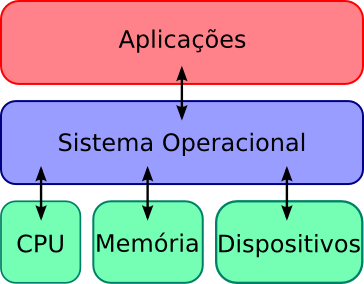
\includegraphics[width=250px]{figuras/OS.png}
    \caption{Diagrama Simplificado das camadas l�gicas de um computador moderno.}
    \label{fig:OS}
  \end{center}
\end{figure}

A segunda fun��o do SO trata do gerenciamento de Recursos de hardware: Enquanto h� apenas um processo rodando no sistema computacional, todos os recursos do mesmo est�o dispon�veis para esse processo. Mas a partir do surgimento da necessidade de se executar dois ou mais processos simultaneamente, h� grande complexidade em se fazer gerenciamento inteligente dos recursos utilizados. Nesse ponto, o SO assume a tarefa, realizando o agendamento de uso de mem�ria, tempo de processamento, e uso de perif�ricos, retirando da aplica��o a responsabilidade de gerenciar os recursos dispon�veis.

\section{Sistemas de Tempo Real}
De maneira simplificada, um sistema de Tempo Real (RT) � aquele que exige, da entidade processadora, um limite restrito de tempo entre a aquisi��o dos dados e a emiss�o da resposta resultante do processamento dos dados aquisitados [\cite{RTbook}].
Isso significa que o processamento deve, necessariamente, acontecer durante um determinado intervalo de tempo, cujo in�cio � determinado pela sa�da do sistema. 

O fato de o processamento n�o ter sido feito r�pido o suficiente, � conhecido como perda de prazo (\textit{deadline miss}). 
A rea��o do sistema � perda do prazo pode ser classificada em dois grupos:
\begin{enumerate}
  \item \textit{Soft Real-Time}: A perda do prazo, mesmo que em poucas situa��es, � indesej�vel, afetando negativamente o resultado do processo. Entretanto, a perda de poucos prazos n�o desestabiliza o sitema;
  \item \textit{Hard Real-Time}: Apenas uma perda de prazo tem consequ�ncias s�rias, podendo inclusive causar instabilidade no sistema, fazendo com que o mesmo se comporte de maneira imprevista.
\end{enumerate}

\section{Sistemas Operacionais de Tempo Real}

A fun��o do Sistema Operacional de Tempo Real (RTOS) �, al�m de oferecer os recursos de um Sistema Operacional, suprir de maneira est�vel as necessidades de sistemas RT. 
Para isso, nele deve ser implementado um agendador de tarefas preemptivo, que possua a capacidade de interromper uma tarefa de menor prioridade para a execu��o de uma tarefa com prioridade maior, sem que seja necess�ria colabora��o da tarefa que estava em execu��o. Isso torna previs�vel o tempo entre a requisi��o da tarefa e o seu t�rmino. 

Dessa maneira, se a tarefa de maior prioridade estiver associada ao sistema RT, todos os recursos de processamento do sistema estar�o dispon�veis para que a tarefa possa ser realizada no menor tempo poss�vel, colocando assim todos os esfor�os da plataforma para realizar a tarefa cr�tica antes do prazo (\textit{Deadline}).

� muito comum medir o desempenho de um RTOS pelo tempo entre a requisi��o originada pelo Sistema de Tempo Real e o in�cio da tarefa de processamento relacionada. Esse tempo � conhecido como lat�ncia do sistema. A lat�ncia representa o intervalo de tempo que o RTOS gasta para detectar o requerimento de tarefa, interromper a tarefa atual e inciar a tarefa de alta prioridade.


		\section{FLOSS: \textit{Free and Open Source Software}}
		
Segundo a \cite{flossDef}, Software Livre � aquele em que todos os usu�rios, legalmente, tem todos os seguintes direitos:
\begin{itemize}
  \item Executar o programa para qualquer prop�sito;
  \item Acesso p�blico ao c�digo fonte;
  \item Alterar o c�digo da maneira desejada;
  \item Distribuir as altera��es realizadas. 
\end{itemize}

Esses direitos impactam de maneira positiva sobre projetos de pequeno porte, pois aproveitando as aplica��es e ferramentas j� implementadas pode-se, com pouco esfor�o, adaptar o Software Livre j� existente para realizar as fun��es desejadas. 
Al�m disso, n�o h� nada que impe�a a venda de produtos com Software Livre embarcado, sendo isso um excelente incentivo para jovens empresas na ind�stria de tecnologia.

Atualmente existem diversas licen�as de Software Livre, sendo que cada uma delas tem suas particularidades.
Algumas delas s�o mais restritivas, como a GPL (GNU \textit{Public Licence} [\cite{gpl}]), na qual consta a exig�ncia de que todas as modifica��es realizadas no c�digo sejam compartilhadas, e que os autores sejam mencionados. Outras licen�as s�o mais permissivas, como a Licen�a BSD (Berkeley \textit{Software Distribution} [\cite{bsd}]), que d� autonomia para que o usu�rio fa�a o que desejar com o c�digo, inclusive transformar suas modifica��es no c�digo em software propriet�rio. 

Nesse trabalho, a grande maioria do software utilizado � licenciado pela GPL, que � normalmente adotada pelas distribui��es Linux.
 
    \section{Linux}
O Linux � um n�cleo de Sistema Operacional compat�vel com a fam�lia de normas IEEE POSIX [\cite{locke2005posix}], e tem vasto suporte a diversas arquiteturas e dispositivos.
Ele � desenvolvido sob o modelo de desenvolvimento de software livre, e tendo sido publicado sobre a licen�a GPL, � considerado atualmente o mais bem sucedido SO livre, podendo ser adquirido gratuitamente pela internet. [\cite{focalinux}].

Devido � sua estabilidade, flexibilidade e padroniza��o, o Linux � hoje usado em diversas aplica��es, marcando forte presen�a em supercomputadores (estando em 462 dos 500 mais potentes do mundo [\cite{top500}]) e tendo crescente aceita��o no mercado de \textit{SmartPhones} [\cite{MobileStat}], onde � representado pelo Google Android.


Al�m das qualidades citadas previamente, o Linux conta com uma documenta��o bastante convidativa e uma boa comunidade de suporte, mostrando-se um SO excelente para o desenvolvimento de aplica��es embarcadas.

  \section{Distribui��es de Software}

O objetivo de uma distribui��o de software � facilitar a instala��o de aplicativos e ferramentas em um sistema operacional.
Isso acontece a partir do uso de um reposit�rio de software, do qual o usu�rio tem a possibilidade de descarregar programas separados em determinadas cole��es. Cada cole��o tem diferentes objetivos: algumas delas prezam por softwares mais atualizados, enquanto outras priorizam a estabilidade do software utilizado.

Algumas distribui��es de software mais conhecidas frequentemente oferecem outros recursos desej�veis:
\begin{itemize}
  \item Gerenciador de Pacotes: � uma ferramenta que automatiza a aquisi��o de pacotes atrav�s do reposit�rio e, geralmente, tem recursos de solu��o de depend�ncia entre pacotes (adquire pacotes necess�rios para o funcionamento do pacote desejado);
  \item Pacotes Bin�rios: A distribui��o oferece os pacotes de software j� pr�-compilados e prontos para o uso.
  \end{itemize}

Com o objetivo de evitar a concentra��o de tr�fego de dados no servidor do reposit�rio, as distribui��es mais conhecidas recebem suporte de espelhos (\textit{mirrors}), que s�o c�pias exatas e verificadas do servidor original.

 \section{Interpretador de Comandos: \textit{Shell}}

A fun��o do interpretador de comandos (\textit{Shell}) �, como o nome deixa claro, interpretar os comandos enviados pelo usu�rio para o OS, servindo assim como interface que torna direta a comunica��o entre estes [\cite{bLp}].

O \textit{Shell} �, at� a data de elabora��o deste trabalho, a principal interface entre os sistemas Linux embarcados e o usu�rio, portanto seu uso � bastante requisitado nesse tipo de projeto. A partir do \textit{Shell} � poss�vel executar diversos aplicativos e utilizar basicamente todas as ferramentas dispon�veis no sistema. 

No intuito de realizar tarefas repetitivas de maneira autom�tica, pode-se fazer um \textit{Shell Script}. Seu funcionamento � simples: basta abrir qualquer editor de texto e escrever os comandos que devem ser realizados, na ordem desejada e separando-os por linha e salv�-los em um arquivo. Feito isto, basta conceder permiss�o para que o sistema operacional use arquivo de \textit{Shell Script} como execut�vel, e as tarefas nele descritas ser�o realizadas automaticamente. Comandos de condi��o (\textit{if, else}) e la�o (\textit{for, while, until}) tamb�m est�o dispon�veis para a constru��o do \textit{script}.

    
\section{Microcontroladores ARM}

ARM (\textit{Advanced RISC Machines}) � uma arquitetura de microprocessadores em crescente desenvolvimento, que conta com as seguintes caracter�sticas [\cite{armBook}]:
\begin{itemize}
  \item Constru�da sobre o Design RISC (\textit{Reduced Instruction Set Computer}) : visa proporcionar um conjunto com comandos reduzido, que sejam mais r�pidos e possam ser organizados de forma a gerar instru��es complexas mais flex�veis;
  \item Alguns Conceitos n�o RISC: Possui chaveamento para realizar algumas instru��es complexas e instru��es estendidas para processamento num�rico de alto desempenho;
  \item Efici�ncia El�trica: Projetada para ter baixo consumo e medidas mec�nicas reduzidas, � ideal para equipamentos m�veis;
  \item Alta Densidade de C�digo: O arquivo execut�vel (bin�rio) ocupa menos espa�o em mem�ria, o que � desej�vel em sistemas mais limitados.
\end{itemize}

Entretanto, para manter o baixo consumo el�trico, a maioria dos processadores ARM n�o disp�em de grande poder de processamento. A gera��o de bin�rios, se realizada nativamente no ARM, pode ser bastante demorada e at� invi�vel. Portanto � pr�tica bastante comum a compila��o cruzada (\textit{Cross-Compiling}), que visa usar m�quinas de maior desempenho a fim de gerar bin�rios que podem ser executados na arquitetura ARM.

\section{Plataforma Embarcada com Linux}

No geral, as plataformas com Linux embarcado cont�m os seguintes componentes de software: 
\begin{figure}[H]
  \begin{center}
    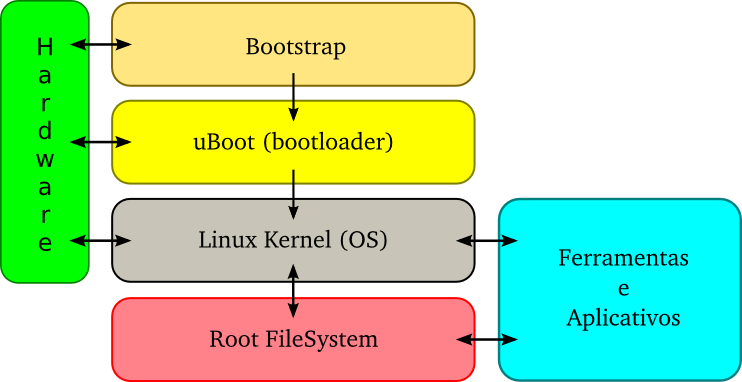
\includegraphics[width=450px]{figuras/Embedded.png}
    \caption{Diagrama Simplificado da comunica��o entre os componentes de uma plataforma com Linux embarcado.}
    \label{fig:embedded}
  \end{center}
\end{figure}
 
\begin{itemize}
  \item \textit{Root FileSystem} (RootFS): � a parti��o onde ficam os arquivos b�sicos do sistema, e geralmente todas as ferramentas e aplica��es dispon�veis pelo sistema. Essa parti��o pode opcionalmente guardar aquivos modificados, e ser usada para descarregar novos softwares. � essencial para o funcionamento do sistema operacional;
  \item \textit{Kernel} Linux: � o n�cleo do SO Linux, onde est�o dispon�veis as principais ferramentas de gerenciamento de hardware;
  \item Gerenciador de Boot (\textit{Bootloader}): Software respons�vel por indicar a localiza��o do \textit{Kernel} e do RootFS, de modo que o OS possa ser iniciado. Alguns \textit{Bootloaders} tem recursos avan�ados como suporte a rede e passagem de vari�veis ao \textit{kernel};
  \item \textit{Bootstrap}: Presente em alguns casos, esse software realiza o carregamento do \textit{Bootloader}.

\end{itemize}


Na Figura \ref{fig:embedded} � mostrada a comunica��o entre os componentes da Plataforma Embarcada com Linux.

\chapter{Materiais e Metodologia}
Este cap�tulo divide a metodologia utilizada em duas sess�es: a primeira apresenta os materiais utilizados, englobando hardware e software. A segunda aborda os m�todos utilizados para a obten��o dos resultados. 

\section{Materiais Usados}
Nesta sess�o s�o apresentados os materiais utilizados na constru��o do trabalho. O principal hardware utilizado foi o Kit de Desenvolvimento SAM9-L9260 (descrito na Se��o ~\ref{sec:kit}), enquanto os principais softwares utilizados foram o c�digo fonte do Linux (Se��o ~\ref{sec:linuxsrc}), o \textit{patch} RT (Se��o ~\ref{sec:patchsrc}) e a ferramenta de testes CyclicTest (Se��o ~\ref{sec:cyclic}).

\subsection{Kit de Desenvolvimento SAM9-L9260}
\label{sec:kit}
Com o intuito de evitar o trabalho relacionado � montagem de hardware, foi adquirido o kit de desenvolvimento da Olimex� SAM9-L9260, que cont�m um microcontrolador ARM embarcado, bem como mem�rias vol�til e NAND Flash. As configura��es mais relevantes ao trabalho est�o descritas a seguir [\cite{kitMan}]:

\begin{itemize}
  \item  MCU AT91SAM9260 de 16/32 bits arquitetura ARM9\texttrademark \ rodando a 200MHz;
  \item  Frequ�ncia principal do sistema igual a 50MHz;
  \item  64 MB SDRAM;
  \item  512MB NAND \textit{Flash} para armazenamento (RootFS);
  \item  Conector \textit{Ethernet} 100Mbit;
  \item  Conectores USB \textit{host} (tipo B) e USB \textit{device} (tipo A);
  \item  Interface Serial (RS232), usada como terminal serial;
  \item  Conector para cart�es de mem�ria SD/MMC;
  \item  \textit{Bootloader} uBoot, e \textit{Bootstrap} j� configurados;
  \item  \textit{Kernel} Linux 2.6.31-rc3 customizado;
  \item  Distribui��o de Software Debian vers�o 4.0 codinome "Etch". 
\end{itemize}

A Figura \ref{fig:SAM} mostra vis�es de perspectiva isom�trica (esquerda) e vis�o de fundo (direita) da placa utilizada.
\begin{figure}[H]
  \begin{center}
    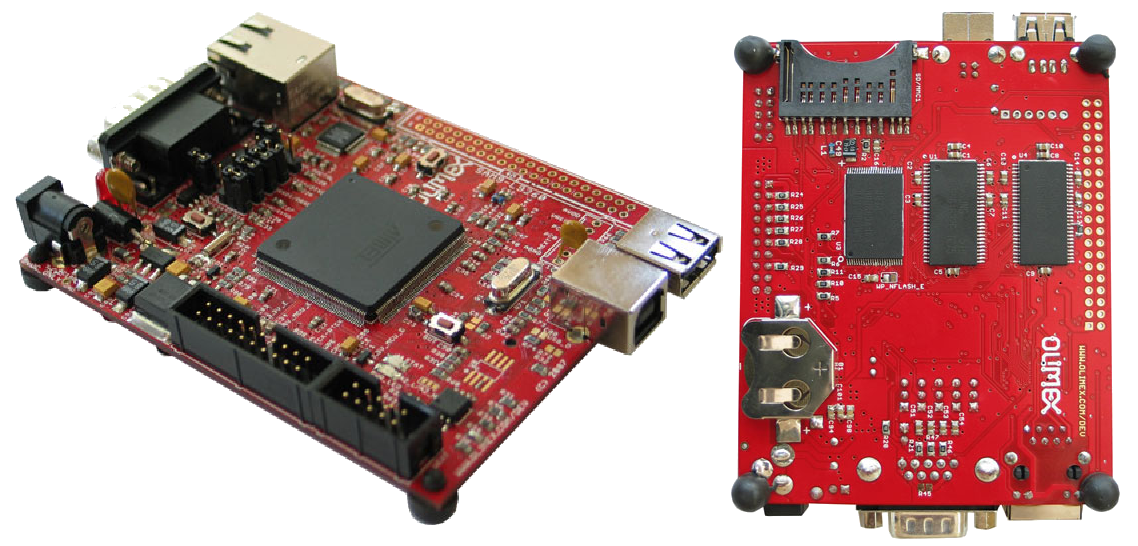
\includegraphics[width=450px]{figuras/olimex.png} 
    \caption{Fotos do Kit SAM9L9260.[\cite{kitMan}] }
    \label{fig:SAM}
  \end{center}
\end{figure}
O \textit{uBoot} permite \textit{download} de kernel via protocolo TFTP (\textit{Trivial File Tranfer Protocol}), e oferece a possibilidade de usar um Root FileSystem (RootFS) a partir de cart�o de mem�ria SD/MMC ou Pendrive (USB \textit{device}) ao inv�s da NAND \textit{Flash} interna.

\subsection{C�digo Fonte do \textit{Kernel} Linux}
\label{sec:linuxsrc}

O c�digo fonte do \textit{Kernel} Linux est� dispon�vel na internet [\cite{linuxSource}]. O download pode ser realizado tamb�m em um dos espelhos disponibilizados nesse mesmo endere�o.
A partir do c�digo foram feitas as modifica��es necess�rias para tornar o Linux um RTOS. 

A vers�o escolhida para a execu��o do trabalho foi a 3.4.9, sendo esta a vers�o mais nova que mantinha compatibilidade com o \textit{patch Real-Time}, considerando o per�odo em que ocorreu a execu��o deste trabalho.

\subsection{\textit{Patch Real Time} para Linux}
\label{sec:patchsrc}
\textit{Patch} � um arquivo que traz algumas modifica��es que podem ser aplicadas ao c�digo fonte de um software para faz�-lo realizar tarefas diferentes, corrigir algum defeito, ou adicionar suporte a novas plataformas. Quando o \textit{patch} atinge um certo n�vel de maturidade e relev�ncia para o projeto original geralmente ele � absorvido e se torna uma op��o de configura��o a mais na hora da compila��o. 

A fun��o desse \textit{patch} � aumentar a preemp��o do Linux, permitindo melhor atendimento das tarefas de alta prioridade. Isso � feito na tentativa de adaptar o Linux para que ele funcione como um Sistema Operacional de Tempo-Real. O \textit{patch} RT � um projeto oficial do Kernel.org e o \textit{Wiki} do projeto est� dispon�vel na internet [\cite{rtpatch}].

\subsection{Ferramenta de Testes \textit{Cyclictest}}
\label{sec:cyclic}
Cyclictest � uma ferramenta usada para levantar estat�sticas sobre os tempos de lat�ncia da plataforma em que � executado. 
Essa ferramenta � recomendada pela comunidade Embedded Linux [\cite{elinux}] como uma boa pr�tica de teste para sistemas RT.

O Cyclictest funciona requerendo, em uma frequ�ncia definida e bastante precisa, que o OS realize uma tarefa de alta prioridade. O tempo de lat�ncia � ent�o calculado e armazenado. Ao final do teste tem-se o valor m�ximo, m�nimo, m�dio e o n�mero de vezes que a tarefa foi requerida.


\section{M�todos Usados}
Nesta sess�o s�o explicados os m�todos utilizados para a obten��o dos resultados, onde as Se��es de \ref{ss:CC} at� \ref{ss:startup} explicam os como foi feita a gera��o e a configura��o da plataforma, enquanto a Se��o \ref{ss:teste} explica os procedimentos de teste.
\subsection{Compila��o Cruzada}
	\label{ss:CC}
Antes de iniciar a explica��o sobre a compila��o cruzada, � necess�rio salientar que em necessidade de executar algum processo como super-usu�rio ou administrador (\textit{root}), os seguintes comandos foram usados antes do in�cio do bloco:


 \begin{lstlisting}
 sudo su  #(sistemas com sudo instalado) ou
 su       #(sistemas sem sudo instalado).
 \end{lstlisting}

Nada impede de que todos os processos sejam executados como root, mas por boa pr�tica ser�o citados aqueles que exigem esse n�vel de privil�gio.

A primeira etapa foi obter o c�digo fonte do \textit{Kernel} Linux e prepar�-lo para aplica��o do patch. Para isso, seguiu-se os seguintes passos:


 \begin{lstlisting}
  # Realiza o Download do Linux vers�o 3.4.9.
  wget http://www.kernel.org/pub/linux/kernel/v3.x/linux-3.4.9.tar.xz
  # Extrai o pacote em uma pasta de mesmo nome:
  tar -xJf linux-3.4.9.tar.xz
  # Para entrar na pasta referente:
  cd linux-3.4.9
  \end{lstlisting}

A pr�xima etapa foi obter o arquivo de \textit{patch} e aplic�-lo ao c�digo do Linux:


 \begin{lstlisting}
# Realiza o Download do Patch RT para o Linux 3.4.9
  wget http://www.kernel.org/pub/linux/kernel/projects/rt/3.4/older/patch-3.4.9-rt17.patch.xz
# Extrai o Patch
  xz -d patch-3.4.9-rt17.patch.xz
# Aplica o patch ao c�digo.
  patch -p1 < patch-3.4.9-rt17.patch 
  \end{lstlisting}


Com esses comandos, o c�digo do Linux foi alterado com as modifica��es propostas pelo \textit{patch}. 
Antes de continuar, foi necess�rio instalar alguns pacotes para possibilitar a compila��o cruzada entre o computador usado e o kit de desenvolvimento. Os comandos a seguir foram usados em distribui��es Debian ou descendentes (como o Ubuntu) que usam gerenciador de pacotes APT (\textit{Advanced Packaging Tool}). Caso seja necess�rio realizar esse processo em outra distribui��o � indicado usar o gerenciador de pacotes da mesma, ou o processo por ela indicado para realizar a instala��o. 


 \begin{lstlisting}
# Os comandos a seguir devem ser executados como Super-Usu�rio.
# Instalando o Compilador Cruzado 
 apt-get install gcc-arm-linux-gnueabi
# Instalando bibliotecas b�sicas para compilar o kernel.
 apt-get install gcc make libncurses-dev
# Instalando bibliotecas necess�rias para usar o configurador gr�fico do kernel. (Opcional)
 apt-get install libqt4-dev
 \end{lstlisting}

Nesse ponto iniciou-se a configura��o do Linux para o kit de desenvolvimento utilizado. A linha 8 gera a configura��o padr�o do kit, e foi obtida em seu manual [\cite{kitMan}].

\newpage
 \begin{lstlisting}
# Limpa qualquer tentativa de compila��o anterior.
 make clean  
# Exporta as vari�veis para a Compila��o Cruzada.
export ARCH=arm
export CROSS_COMPILE=arm-linux-gnueabi-

# Aplica a configura��o de compila��o padr�o do Kit.
  make sam9_l9260_defconfig
# Para configurar o Linux com a ferramenta gr�fica:
  make xconfig
# Para configurar o Linux com a ferramenta de texto:
  make menuconfig
 \end{lstlisting}

Para a configura��o deste Kit foi necess�rio adicionar configura��es espec�ficas, sendo algumas para funcionamento em geral e outras para o funcionamento em Real-Time. Para mais detalhes veja o Ap�ndice \ref{ap:kernel}.

Uma vez acabados os ajustes, foram executados os seguintes comandos para realizar a compila��o do Linux e a sua c�pia para a pasta atual:


 \begin{lstlisting}
# Realiza a compila��o, usando os 4 n�cleos do processador para reduzir o tempo,
  make uImage -j4
# Move o Linux compilado para o diret�rio atual,
  mv arch/arm/boot/uImage .
 \end{lstlisting}
 
   Para finalizar, foi necess�rio mover o arquivo uImage para um servidor de TFTP(\textit{Trivial File Tranfer Protocol}), de onde ele pudesse ser obtido pelo \textit{uBoot}. O endere�o IP do servidor era 10.235.0.130. Para mais detalhes, veja o Ap�ndice \ref{ap:tftp}.
  

\subsection{Cria��o do \textit{Root FileSystem}}
	\label{ss:rootfs}
Para a cria��o do \textit{Root FileSystem} (RootFS) foi usada uma ferramenta da Distribui��o Debian (que tamb�m est� presente nas distribui��es descendentes) chamada Debootstrap. Esta ferramenta usa os reposit�rios da distribui��o Debian (ou descendentes) para montar um RootFS b�sico. 
 Al�m desta, foi necess�rio instalar algumas ferramentas de emula��o para concluir a configura��o do Debian, de modo a transferir o RootFS pronto para o Kit. Os procedimentos de configura��o s�o mostrado nos trechos de c�digo a seguir:


 \begin{lstlisting}
# Os comandos a seguir devem ser executados como Super-Usu�rio.
#Instala o Debootstrap e os emuladores (qemu).
 apt-get install binfmt-support qemu qemu-user-static debootstrap
 \end{lstlisting}


Ap�s o t�rmino da instala��o, via APT, do Debootstrap e das ferramentas de emula��o, criou-se uma pasta onde foi feito o processo do Debootstrap. O processo foi realizado como mostrado a seguir:


 \begin{lstlisting}
# Os comandos a seguir devem ser executados como Super-Usu�rio.
# Criando e entrando na pasta usada no Debootstrap:
 mkdir Debootstrap
 cd Debootstrap
# Usando o Debootstrap para criar, na pasta debian, um RootFS da Vers�o Wheezy (7.0) usando a arquitetura armel (ARM),a partir do espelho da USP do reposit�rio Debian.
 debootstrap --foreign --arch armel wheezy debian/ http://sft.if.usp.br/debian/
\end{lstlisting}

O pr�ximo passo foi usar a pasta debian como RootFS e realizar a emula��o da plataforma ARM para terminar a configura��o. Para isso, foi necess�rio copiar o emulador para dentro da pasta debian, pois caso contr�rio a emula��o falharia:

 \begin{lstlisting}
# Os comandos a seguir devem ser executados como Super-Usu�rio.
# Copia o emulador para a pasta debian.
  cp /usr/bin/qemu-arm-static debian/usr/bin/
# O comando a seguir exporta algumas variaveis e usa o comando chroot para iniciar a emula��o de um Microcontrolador ARM.
  DEBIAN_FRONTEND=noninteractive DEBCONF_NONINTERACTIVE_SEEN=true LC_ALL=C LANGUAGE=C LANG=C chroot debian/

# Dentro da emula��o, instala-se todos os pacotes DEB baixados com o comando debootstrap
dpkg --force-all -i /var/cache/apt/archives/*.deb

# Caso ocorra algum erro na configura��o do base-files. comente esta linha (coloque um # antes de rmdir) para corrigir o bug.
# O comando a seguir o levar� diretamente na linha 30, que precisa ser comentada.
  nano +30 /var/lib/dpkg/info/base-files.postinst 
# ctrl+o para salvar e ctrl+x para sair.
 \end{lstlisting}


Para possibilitar o uso do APT, adicionou-se os endere�os dos reposit�rios de onde poderia ser feita a aquisi��o de pacotes. O reposit�rio escolhido foi o da USP por se mostrar com maior taxa de transfer�ncia dentro do campus. O procedimento � mostrado a seguir:

 \begin{lstlisting}
# Adiciona o reposit�rio SFT da USP na lista de reposit�rios.
  echo "deb http://sft.if.usp.br/debian wheezy main contrib non-free" > /etc/apt/sources.list
# Baixa a listagem do reposit�rio e realiza as atualiza��es, al�m de corrigir os poss�veis problemas com o base-files.
  apt-get update && apt-get dist-upgrade -y
#Para sair da emula��o, use o comando exit
exit
 \end{lstlisting}
Ap�s terminada a emula��o, a pasta debian continha todos os recursos b�sicos para, juntamente com um kernel, iniciar o sistema operacional. 
Por fim, foram transferidos os conte�dos da pasta debian para um \textit{pendrive}, que foi usado no processo de \textit{boot}.

 \begin{lstlisting}
# Os comandos a seguir devem ser executados como Super-Usu�rio.
# Formata (em EXT3) o pendrive (/dev/sdb) 
  mkfs.ext3 -L "pendrive"  /dev/sdb
# Monta o pendrive na pasta /media/pendrive
  mount -t ext3 /dev/sdb /mnt/
# Copia conte�do do RootFS para o pendrive.
  cp -r debian/* /mnt/
  umount /dev/sdb
 \end{lstlisting}
	
\subsection{Iniciando o Sistema}
\label{ss:startup}
  
Foi necess�rio conectar, atrav�s de um cabo serial, o kit e um computador de mesa a fim de usar um emulador de terminal serial (Minicom, Teraterm) para alterar as configura��es do \textit{uBoot}. O emulador foi ajustado nas seguintes configura��es:
  
  \begin{itemize}
    \item \textit{Baud Rate}: 115200;
    \item Bits de Dados: 8;
    \item \textit{Stop} Bits: 1;
    \item Sem controle de fluxo.
  \end{itemize}

Ao ligar a placa, apareceu a op��o de cancelar o \textit{boot} autom�tico. Quando cancelado, foi mostrado o terminal do \textit{uBoot}, onde foram feitas as configura��es para realizar o \textit{boot} a partir do Kernel presente no servidor TFTP e o RootFS do \textit{pendrive}. Uma vez que o arquivo \textit{uImage} j� estava no servidor TFTP e o \textit{pendrive} j� havia sido constru�do, bastou inserir-lo na entrada USB da placa (USB \textit{device}), conectar o cabo de rede e usar os seguintes comandos de configura��o (adaptados de [\cite{kitMan}]):

  \begin{lstlisting}
# Aponta o local do servidor 
  setenv serverip 10.235.0.130
# Atribui o endere�o local
  setenv ipaddr 10.235.0.136
# Descarrega o uImage via TFTP e o carrega no endere�o 0x22200000
  tftpboot 22200000 10.235.0.130:uImage
# Ajusta a localiza��o do RootFS para o pendrive (/dev/sda1)
  setenv bootargs mem=64M console=ttyS0,115200 root=/dev/sda rootdelay=10
# Realiza o Boot
  bootm
 \end{lstlisting}

Foi ent�o realizado o \textit{boot} da maneira desejada e o Sistema Operacional iniciou como esperado. Para listar as caracter�sticas do mesmo foi usado o comando \textit{uname}:


  \begin{lstlisting}
# Comando para listar caracter�sticas do OS, 
  uname -a
# Retorno
"Linux SAM9-L9260 3.4.9-rt17 #11 PREEMPT RT Mon Sep 10 17:25:28 BRT 2012 armv5tejl GNU/Linux"
 \end{lstlisting}

 A partir destas listagens pode-se verificar que o processo de constru��o do Linux RT ocorreu com sucesso.
 

\subsection{Testes de Desempenho}	
Nesta Se��o s�o detalhados os procedimentos de teste utilizados para demonstrar as caracter�sticas obtidas pelo Linux ap�s a configura��o e a aplica��o do \textit{patch} RT.

  \label{ss:teste}
	\subsubsection{Teste de \textit{Clock}}

O teste de \textit{clock} foi um teste que teve por objetivo de verificar a diferen�a ocasionada pelo uso do comando \textit{chrt} no comportamento do ambiente em diferentes situa��es. 

A fun��o do comando \textit{chrt} � manipular os atributos RT de um processo, aumentando ou diminuindo a sua prioridade de execu��o. Atrav�s dele � poss�vel selecionar os processos que ser�o vinculados ao sistema de tempo real, e portanto ser�o priorit�rios [\cite{siever2009linux}].

O teste gerava sinal de \textit{clock} a partir de um pino de GPIO(\textit{General Purpose Input Output} - Pino de uso geral) o mais r�pido poss�vel. Com o aux�lio de um oscilosc�pio, mediu-se o per�odo de meia onda, que representa o tempo de chaveamento do GPIO.

Para isso, dois meios foram propostos para gerar o sinal: \textit{Bash Script} e um programa escrito em linguagem C.
Cada um desses meios foi testado de tr�s maneiras:
\begin{enumerate}
  \item Usando o Linux com o \textit{patch} RT, sem alterar a prioridade da tarefa, que tem o mesmo resultado do Linux sem o \textit{patch} RT;
  \item Usando o Linux sem o \textit{patch} RT,  alterando a prioridade da tarefa para o m�ximo (\textit{chrt});
  \item Usando o Linux com o \textit{patch} RT, alterando a prioridade da tarefa para o m�ximo (\textit{chrt}).
\end{enumerate}

A partir desses valores foi poss�vel perceber a influ�ncia do \textit{patch} nas temporiza��es do Linux, e tamb�m os efeitos provocados pelo comando \textit{chrt} no comportamento do Linux. Os tempos observados nesses testes foram referenciados como "per�odos de meia onda", e equivalem ao tempo que leva ao ambiente realizar uma troca de valores em um GPIO.
Os detalhes sobre a codifica��o do teste podem ser encontrados no Ap�ndice \ref{ap:clk}.

  \subsubsection{Teste de Lat�ncia por GPIO}

Esse teste j� foi um pouco mais elaborado, e teve por objetivo encontrar, no kit testado, o tempo entre a recep��o de um sinal por um pino de entrada e a resposta a esse sinal por um pino de sa�da. Esse tempo � denominado tempo de resposta do ambiente. 

O sinal de entrada era proveniente do pino de GPIO de um Kit Auxiliar, e tinha a forma de onda quadrada com per�odo de 2ms. A resposta aparecia a cada borda de transi��o do sinal de entrada, e era dada na forma de um pulso. Ambas entrada e sa�da foram colocadas nos dois canais de um oscilosc�pio, que foi colocado em modo de persist�ncia infinita de imagem, e teve o \textit{trigger} fixado nas bordas de transi��o da entrada. Isso ocasionou que todos os pulsos de sa�da fossem marcados na imagem, possibilitando a medida dos tempos de resposta. O diagrama de montagem do teste � representado na Figura \ref{fig:gpiotest}.

\begin{figure}[H]
  \begin{center}
    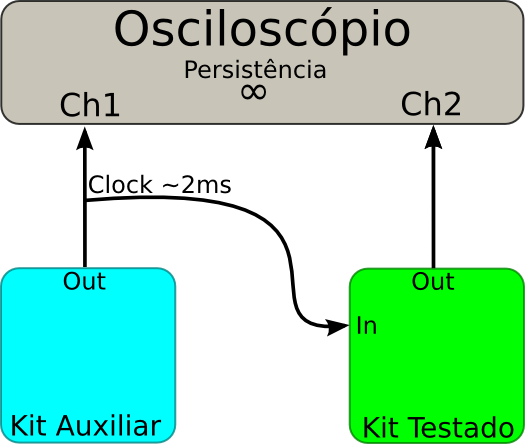
\includegraphics[width=250px]{figuras/teste_gpio.png}
    \caption{Diagrama de Montagem do teste de GPIO.}
    \label{fig:gpiotest}
  \end{center}
\end{figure}



O teste foi aplicado em duas vers�es do Linux: uma com o \textit{patch} RT, e a outra sem o \textit{patch} RT, sendo que em cada vers�o o teste foi feito com o ambiente sobrecarregado de tarefas e repetido com opera��o em baixa carga.

Esse teste foi muito importante, por representar uma situa��o real�stica de aplica��o da plataforma para automa��o.

Atrav�s de experi�ncias emp�ricas, percebeu-se que infelizmente o teste n�o poderia ter dura��o muito longa, j� que este utilizava a fun��o de persist�ncia de imagem no oscilosc�pio. Assim, a imagem poderia ser borrada por perda de sincronia, ocasionada por algumas oscila��es na rede, ou quaisquer fatores externos. 

Os tempos observados nesses testes ser�o referenciados como "tempos de resposta", e s�o referentes � soma dos tempos de lat�ncia e de altern�ncia de n�vel no pino do GPIO.

Mais detalhes sobre a constru��o do teste encontram-se no Ap�ndice \ref{ap:gpio}. 
		
  \subsubsection{\textit{CyclicTest}}
  
  Antes de usar o \textit{CyclicTest}, melhor explicado na sess�o \ref{sec:cyclic} , foi necess�rio obter o c�digo fonte dos reposit�rios \textit{Kernel.org} e compil�-lo no Kit j� em funcionamento. O processo de compila��o � simples e pode ser visto no Ap�ndice \ref{ap:cycl}.
  
  Uma vez compilado e instalado, o CyclicTest foi chamado da seguinte maneira:
  
     \begin{lstlisting}
  time cyclictest -m -a -t -n -p99
 \end{lstlisting}
	
Onde:
\begin{itemize}
  \item \textit{time}: Comando que executa o comando a seguir e retorna o tempo levado para sua execu��o;
  \item -m : Trava as aloca��es de mem�ria da maneira atual. Necess�rio para evitar erros de Segmenta��o;
  \item -a : Indica para todos os testes serem feitos com processador 1;
  \item -t : Usa uma \textit{thread} por processador, pois o sistema possui apenas 1 \textit{thread};
  \item -n : Faz a temporiza��o com a fun��o \textit{nanosleep()}, que � mais precisa;
  \item -p99 : Aumenta a prioridade do teste ao m�ximo, ou seja, o mesmo n�o pode ser interrompido, e sempre interrompe qualquer outra tarefa.
\end{itemize}

Por padr�o, o \textit{CyclicTest} executa um teste a cada 1ms e usa cada tempo medido para realizar as estat�sticas do teste.

\chapter{Resultados}
\label{ch:res}
Este cap�tulo apresenta os resultados dos testes apresentados no Cap�tulo 3. A Se��o \ref{sec:clkr} apresenta os resultados dos testes de \textit{clock}. Na Se��o \ref{sec:gpior} s�o apresentados os resultados dos testes de GPIO. J� a Se��o \ref{sec:cycr} apresenta os resultados do \textit{CyclicTest}.

Note que nos resultados dos testes mostrados da Figura \ref{fig:bclknrt} at� a Figura \ref{fig:crt-l} deve-se verificar as medidas de tempo utilizando os valores dos cursores a direita de cada figura, onde s�o representados pela vari�vel $\Delta  X$, visto que a escala de cada imagem foi ajustada para preservar a riqueza de detalhes.

\section{Teste de \textit{Clock}}
\label{sec:clkr}
O teste de \textit{clock} foi realizado de duas maneiras: uma por \textit{Bash-Script}, mostrado na primeira Se��o, e outra por um execut�vel escrito em linguagem C, mostrado na segunda Se��o.\\ A constu��o de ambos os testes � mostrada no Ap�ndice \ref{ap:clk}.

\subsection{\textit{Clock} em \textit{Bash-Script}}

A Figura \ref{fig:bclknrt} � resultado do programa \textit{bash-clock} rodado no Linux com \textit{patch} RT, a partir do seguinte comando:
  \begin{lstlisting}
./bash-clock
 \end{lstlisting}

	\begin{figure}
	  \begin{center}
	    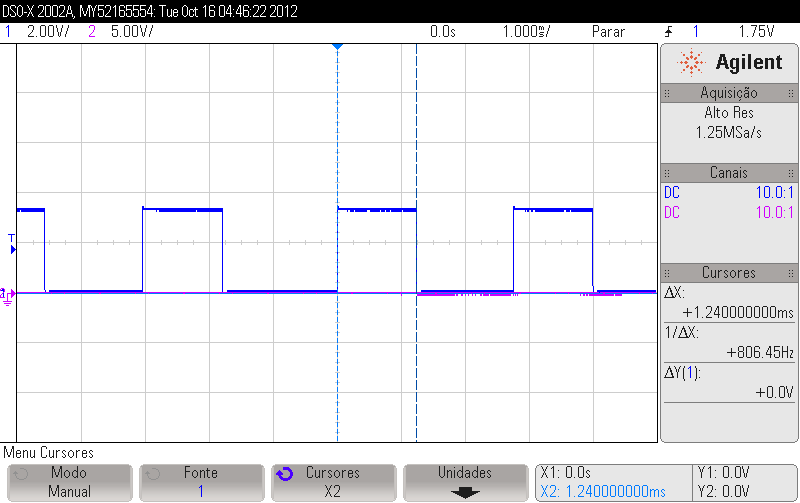
\includegraphics[width=400px]{figuras/clk_bash_srt.png}
	    \caption{\textit{Clock} via \textit{Bash-Script} no Linux com o \textit{patch} RT.}
	    \label{fig:bclknrt}
	  \end{center}
	\end{figure}
 
A Figura \ref{fig:bclknon} �  resultado do programa \textit{bash-clock} rodado no Linux sem o \textit{patch} RT, a partir do comando:
  \begin{lstlisting}
chrt -f 99./bash-clock
 \end{lstlisting}

 A Figura \ref{fig:bclkrt}, � fruto do programa \textit{bash-clock} rodado no Linux com \textit{patch} RT a partir do seguinte comando:
  \begin{lstlisting}
  chrt -f 99 ./bash-clock
 \end{lstlisting}

 
	\begin{figure}
	  \begin{center}
	    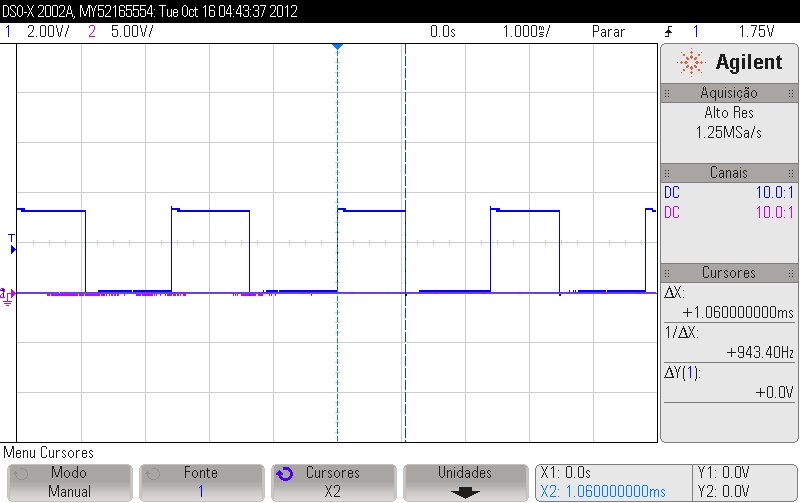
\includegraphics[width=400px]{figuras/clk_bash_non.png}
	    \caption{\textit{Clock} via \textit{Bash-Script} no Linux sem o \textit{patch} RT, com \textit{chrt}.}
	    \label{fig:bclknon}
	  \end{center}
	\end{figure}


	\begin{figure}
	  \begin{center}
	    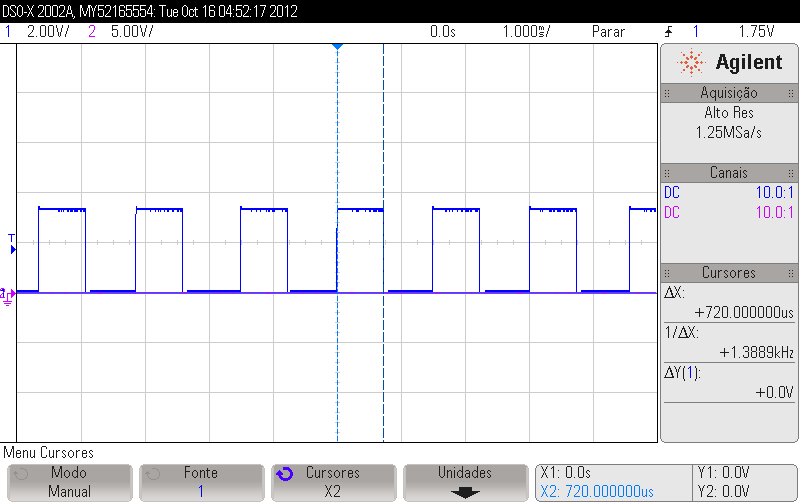
\includegraphics[width=400px]{figuras/clk_bash_crt.png}
      \caption{\textit{Clock} via \textit{Bash-Script} no Linux com o \textit{patch} RT, usando \textit{chrt}.}
 	    \label{fig:bclkrt}
	  \end{center}
	\end{figure}

Todos os resultados do teste de \textit{clock} escrito em Bash-Script est�o concentrados na tabela \ref{clktabb}.

\begin{table}[H]
      \centering
      \caption{Resultados do Teste de Clock - \textit{Bash-Script}} 
      \begin{tabular}{cccc}
      \hline
                & Ambiente & \textit{Bash-Script} \\
                \hline
              A & Linux + patch RT (sem chrt) & 1240 us  \\
              B & Linux - patch RT (com chrt) & 1060 us \\
              C & Linux + patch RT (com chrt) & 720 us  \\
              \hline
              \hline
                & Comparativo &  \\
                \hline
                & B/A & 85,4\%  \\
                & C/A & 58,0\%  \\
                & C/B & 67,9\%  \\
      \hline 
      \end{tabular}
      \label{clktabb}
\end{table}

Pode-se verificar, a partir das figuras apresentadas, que o uso do \textit{chrt} reduz os per�odos de semi-ciclo, e que o efeito � mais expressivo no caso do teste usando chrt, mostrado na Figura \ref{fig:bclkrt}, onde o valor equivale a menos de 60\% do tempo da execu��o sem o uso do comando \textit{chrt}, conforme mostra a Figura \ref{fig:bclknrt}. Sabendo que o processo executado era exatamente o mesmo em todos os casos, pode-se confirmar que o \textit{chrt} produz melhores resultados evitando que a tarefa de \textit{clock} seja interrompida por outras tarefas.

%%%%%%%%%%%%%%%%%%%%%%%%%%%%%%%%%%%%%%%%%%%%%%%%%%%%%%%%%%%%%%%%%

\subsection{\textit{Clock} escrito em Linguagem C}


A Figura \ref{fig:clknrt} � resultado do programa \textit{c-clock} rodado no Linux com \textit{patch} RT, a partir do seguinte comando:
  \begin{lstlisting}
./c-clock
 \end{lstlisting}
 
 
A Figura \ref{fig:clknon} � resultado do Teste de \textit{Clock} para o Linux sem o \textit{patch} RT, a partir do comando:
  \begin{lstlisting}
chrt -f 99./c-clock
 \end{lstlisting}


	A Figura \ref{fig:clkrt}, � fruto do programa \textit{c-clock} rodado no Linux com \textit{patch} RT a partir do seguinte comando:
  \begin{lstlisting}
  chrt -f 99 ./c-clock
 \end{lstlisting}

	

			\begin{figure}[H]
	  \begin{center}
	    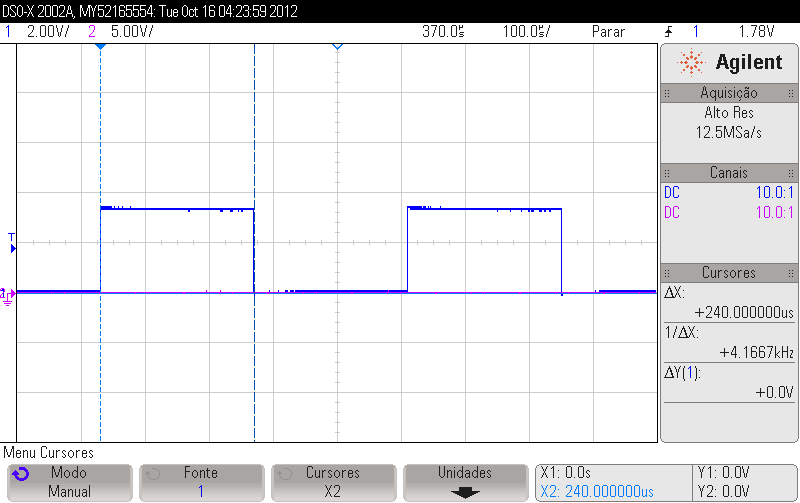
\includegraphics[width=400px]{figuras/clk_csrt.png}
	    \caption{\textit{Clock} escrito em Linguagem C, no Linux com o \textit{patch} RT.}
	    \label{fig:clknrt}
	  \end{center}
	\end{figure}
	
	\begin{figure}[H]
	  \begin{center}
	    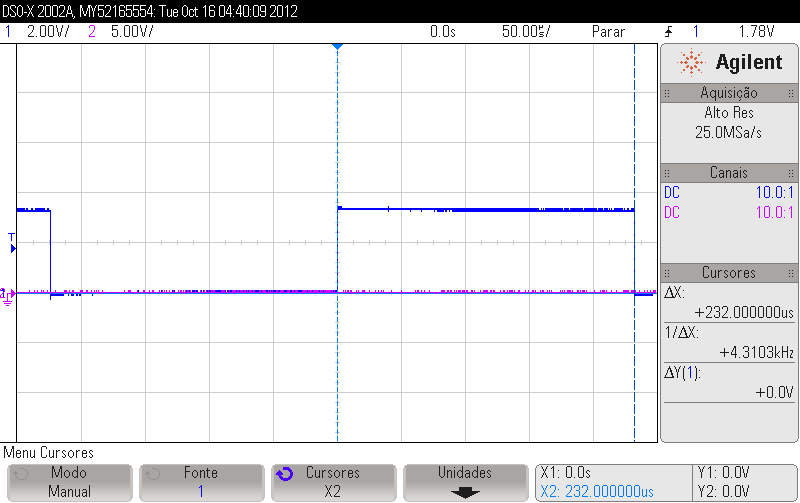
\includegraphics[width=400px]{figuras/clk_srt_non.png}
	    \caption{\textit{Clock} escrito em Linguagem C, no Linux sem o \textit{patch} RT, usando \textit{chrt}.}
	    \label{fig:clknon}
	  \end{center}
	\end{figure}

	\begin{figure}[H]
	  \begin{center}
	    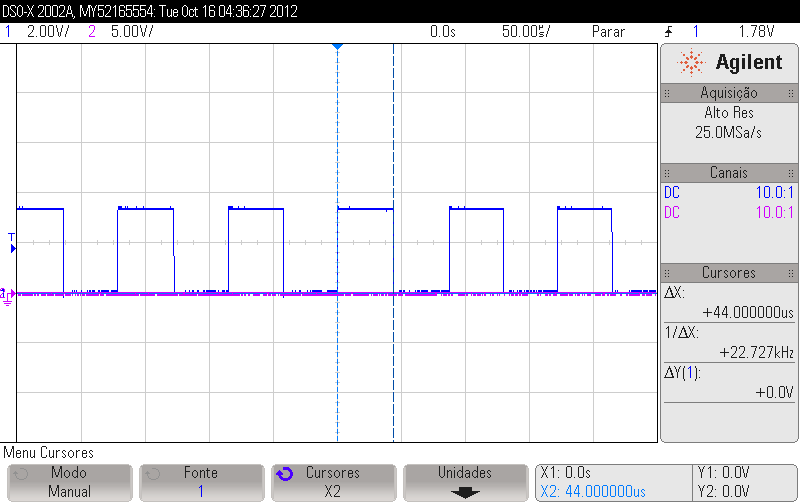
\includegraphics[width=400px]{figuras/clk_crt.png}
	    \caption{\textit{Clock} escrito em Linguagem C, no Linux com o \textit{patch} RT, usando \textit{chrt}.}
	    \label{fig:clkrt}
	  \end{center}
	\end{figure}

Todos os resultados do teste de \textit{clock} escrito em Linguagem C est�o concentrados na tabela \ref{clktabc}.

\begin{table}[H]
      \centering
      \caption{Resultados do Teste de Clock - Linguagem C} 
      \begin{tabular}{ccc}
      \hline
                & Ambiente &  Linguagem C  \\
                \hline
              A & Linux + patch RT (sem chrt) & 240 us \\
              B & Linux - patch RT (com chrt) & 232 us \\
              C & Linux + patch RT (com chrt) & 44 us \\
              \hline
              \hline
                & Comparativo &  \\
                \hline
                & B/A  & 96,7\% \\
                & C/A  & 18,3\% \\
                & C/B  & 19,0\% \\
      \hline 
      \end{tabular}
      \label{clktabc}
\end{table}

Atrav�s destes testes de \textit{Clock}, pode-se notar a aplica��o escrita em C tem uma efici�ncia maior, pelo fato de que o teste em \textit{Bash-Script} realiza a abertura e fechamento do \textit{file-descriptor} do GPIO a cada mudan�a de n�vel, enquanto o teste escrito em C realiza a abertura do \textit{file descriptor} apenas uma vez no in�cio do programa. Isso significa uma boa redu��o de chamadas do sistema e explica a redu��o dr�stica nos valores de tempo de meia-onda.

Pode-se verificar tamb�m que, novamente,  apesar de tamb�m aparecer no Linux sem \textit{patch} RT (Figura \ref{fig:clknon}),  a redu��o no tempo de semi-ciclo foi mais dr�stica no caso do Linux com \textit{patch} RT (Figura \ref{fig:clkrt}), atingindo o valor menor que 20\% do total percebido no mesmo ambiente sem o uso de \textit{chrt}.

� importante ressaltar que, ap�s a chamada do comando com \textit{chrt}, no caso do Linux com \textit{patch} RT, o Sistema Operacional parou de responder, indicando que toda a prioridade de execu��o havia sido dada ao programa de teste, a ponto de n�o haver condi��es de o Sistema Operacional atender os requerimentos do usu�rio.

%%%%%%%%%%%%%%%%%%%%%%%%%%%%%%%%%%%%%%%%%%%%%%%%%%%%%%%%%%%%%%%%%%%


\section{Teste de Lat�ncia por GPIO}
\label{sec:gpior}
O teste de lat�ncia foi aplicado a  dois ambientes distintos: O primeiro ambiente, descrito na Se��o \ref{sub:noload}, opera com baixa carga de processamento, e portanto h� pouca concorr�ncia entre tarefas. O segundo ambiente, descrito na Se��o \ref{sub:load}, opera com sobrecarga de processamento, e portanto h� mais concorr�ncia entre tarefas.

\subsection{Ambiente operando com Baixa Carga de processamento}
\label{sub:noload}

A Figura \ref{fig:srt-n} � resultado do Teste de GPIO no ambiente Linux com \textit{patch} RT rodado pelo seguinte comando:
  \begin{lstlisting}
  chrt -f 99 ./gpio-test
 \end{lstlisting}



A Figura \ref{fig:crt-n} � resultado do Teste de GPIO no ambiente Linux sem \textit{patch} RT rodado pelo seguinte comando:
  \begin{lstlisting}
  chrt -f 99 ./gpio-test
 \end{lstlisting}
	
	\begin{figure}[H]
	  \begin{center}
	    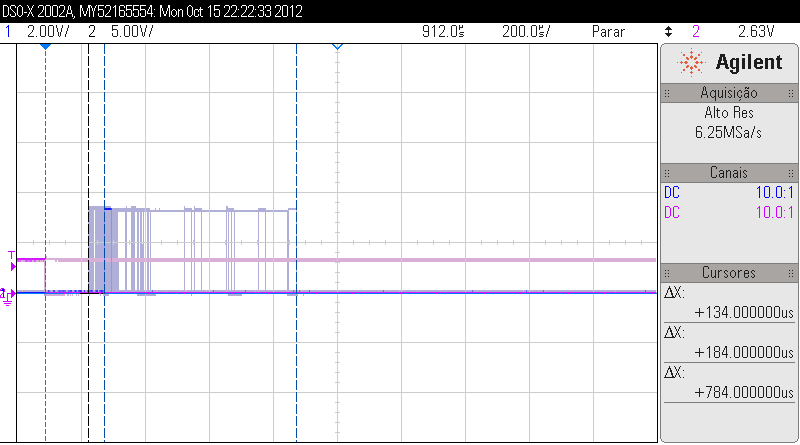
\includegraphics[width=400px]{figuras/nrt_n-comp.png}
	    \caption{Teste por GPIO, com baixa carga, no Linux sem o \textit{patch} RT.}
	    \label{fig:srt-n}
	  \end{center}
	\end{figure}
	\begin{figure}[H]
	  \begin{center}
	    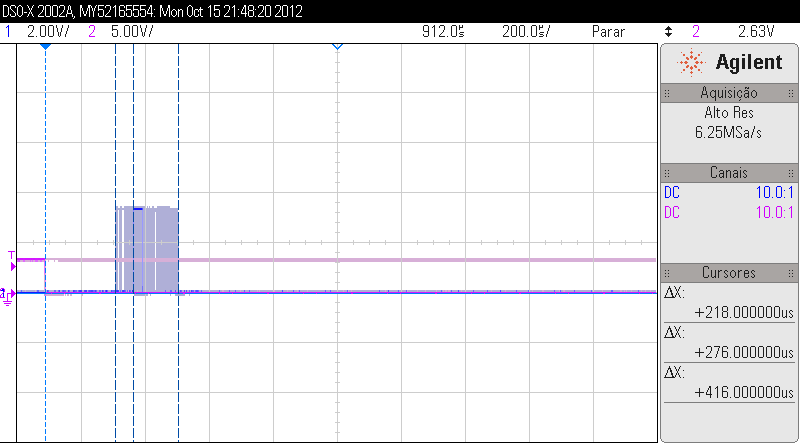
\includegraphics[width=400px]{figuras/rt_n-comp.png}
	    \caption{Teste por GPIO, com baixa carga, no Linux com o \textit{patch} RT.}
	    \label{fig:crt-n}
	  \end{center}
	\end{figure}
	
Os resultados do teste em baixa carga est�o concentrados na tabela \ref{tabgpion}.
	\begin{table}[H]
      \centering
      \caption{Resultados do Teste de Lat�ncia por GPIO - Baixa Carga} 
      \begin{tabular}{cccc}
      \hline
                & Ambiente & Lat�ncia M�nima & Lat�ncia Maxima  \\
                \hline
              A & Linux padr�o & 134 us & 784 us \\
              B & Linux com o patch RT & 218 us & 416 us \\
              \hline
              \hline
                & Comparativo & & \\
                \hline
                & B/A & 162,7\% & 53,0 \% \\
               
      \hline 
      \end{tabular}
      \label{tabgpion}
\end{table}
	
	Como o bin�rio rodado era o mesmo, pode-se perceber que a previsibilidade do tempo de resposta da Figura \ref{fig:srt-n} � bastante inferior � da \ref{fig:crt-n}, que apresentou um tempo m�ximo de resposta muito mais elevado. Isso ocorre porque, mesmo com o \textit{chrt}, o ambiente sem o \textit{patch} RT n�o tem as condi��es de evitar que a tarefa  seja interrompida por outras. J� o ambiente com \textit{patch} RT j� mostra resultados mais condizentes com as necessidades de um Sistema de Tempo-Real.

	



%%%%%%%%%%%%%%%%%%%%%%%%%%%%%%%%%%%%%%%%%%%%%%%%%%%%%%%%%%%%%%%%%%%%

\subsection{Ambiente operando com Sobrecarga de processamento}
\label{sub:load}
O algoritmo que gera a carga no ambiente pode ser encontrado no Ap�ndice \ref{ap:load}. Ele � executado antes do comando de teste, como ser� mostrado a seguir. 

A Figura \ref{fig:srt-l} � resultado do Teste de GPIO no ambiente Linux com \textit{patch} RT, com algoritmo de sobrecarga, rodado pelo seguinte comando:

  \begin{lstlisting}
  ./doload.sh 65 &; chrt -f 99 ./gpio-test
# O primeiro comando (antes do ';') � o algoritmo de carga, e ele � rodado em segundo plano, evidenciado pelo uso do &.
 \end{lstlisting}

A Figura \ref{fig:crt-l} � resultado do Teste de GPIO no ambiente Linux sem \textit{patch} RT, com algoritmo de sobrecarga, rodado pelo seguinte comando:
 
  \begin{lstlisting}
  ./doload.sh 65 &; chrt -f 99 ./gpio-test
 \end{lstlisting}

	\begin{figure}[H]
	  \begin{center}
	    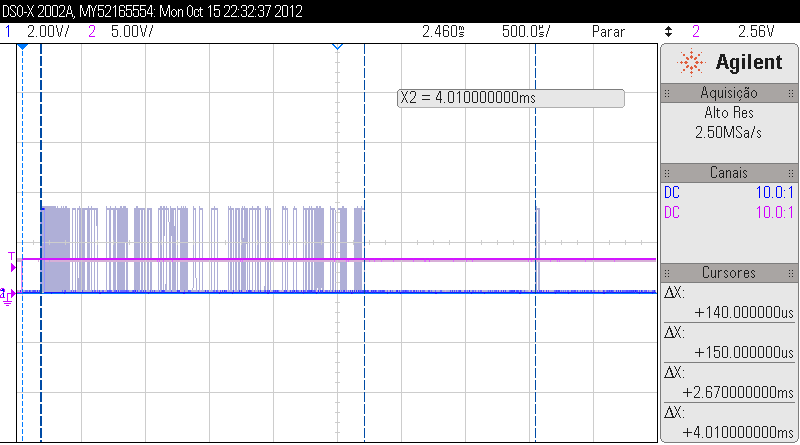
\includegraphics[width=400px]{figuras/nrt_l-comp.png}
	    \caption{Teste por GPIO, com sobrecarga, no Linux sem o \textit{patch} RT.}
	    \label{fig:srt-l}
	  \end{center}
	\end{figure}
	\begin{figure}[H]
	  \begin{center}
	    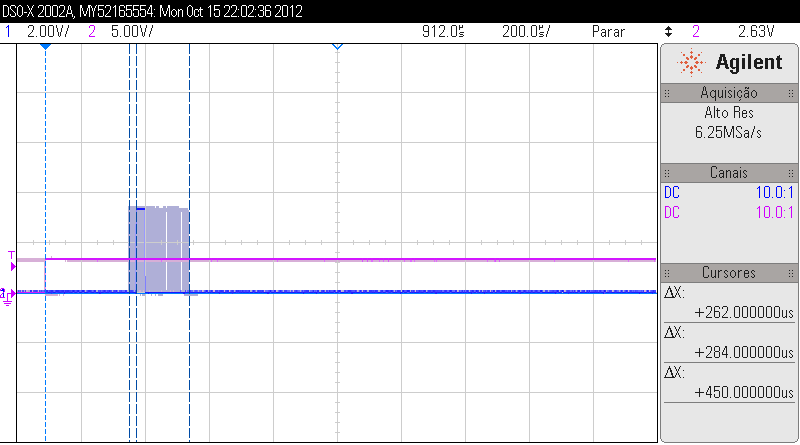
\includegraphics[width=400px]{figuras/rt_l-comp.png}
	    \caption{Teste por GPIO, com sobrecarga, no Linux com o \textit{patch} RT.}
	    \label{fig:crt-l}
	  \end{center}
	\end{figure}


Os resultados do teste em sobrecarga est�o concentrados na tabela \ref{tabgpiol}.

	\begin{table}[H]
      \centering
      \caption{Resultados do Teste de Lat�ncia por GPIO - Sobrecarga} 
      \begin{tabular}{cccc}
      \hline
                & Ambiente & Lat�ncia M�nima & Lat�ncia Maxima  \\
                \hline
              A & Linux padr�o & 140 us & 4000 us \\
              B & Linux com o patch RT & 262 us & 450 us \\
              \hline
              \hline
                & Comparativo & & \\
                \hline
                & B/A & 187,1,7\% & 11,3\% \\
               
      \hline 
      \end{tabular}
      \label{tabgpiol}
\end{table}

� bem simples visualizar que a previsibilidade de tempos de resposta do ambiente com o \textit{patch} RT � muito mais elevada do que a do ambiente sem o \textit{patch}. Isso fica mais evidente no ambiente com sobrecarga, pois a quantidade de tarefas concorrendo com o teste realizado cresce, ocasionando que o teste no ambiente sem o \textit{patch} RT seja interrompido mais vezes do que quando n�o h� carga. J� no ambiente com o \textit{patch} n�o h� necessidade de preocupa��es com a carga, j� que a tarefa de teste tem a maior prioridade poss�vel. 



Em um caso pr�tico, a tarefa de teste � substitu�da pela tarefa cr�tica do Sistema de Tempo Real, que precisa ser atendida dentro de um prazo definido. O ambiente com o \textit{patch} RT sempre seria capaz de atender a tarefa se o prazo fosse menor que 500us, mesmo quando houvesse sobrecarga no sistema. J� o ambiente sem o \textit{patch} teria perdido v�rios prazos e poderia ter levado � instabilidade do sistema de Tempo Real. 
	
	
%%%%%%%%%%%%%%%%%%%%%%%%%%%%%%%%%%%%%%%%%%%%%%%%%%%%%%%%%%%%%%%%%%%%%%%	
\section{\textit{CyclicTest}} %%%%%%%%%%%
\label{sec:cycr}

Para o experimento, dois Kits foram carregados com o mesmo RootFS, e dois Linux diferentes, sendo um deles com o \textit{patch} RT e o outro sem. Ambos os sistemas foram acessados via acesso remoto (SSH - \textit{Secure Shell}) por terminais diferentes, como mostrado abaixo:
 
  \begin{lstlisting}
# No Terminal #1, kit sem patch RT.
  ssh root@10.235.0.135
# No Terminal #2, kit com patch RT.
  ssh root@10.235.0.136
 \end{lstlisting}
 
 Em cada um dos terminais, foram solicitadas duas tarefas de cada placa, sendo a primeira com o objetivo de listar as caracter�sticas do ambiente e outra o pr�prio \textit{CyclicTest}. Os comandos para tal s�o mostrados a seguir:

  \begin{lstlisting}
# Lista caracter�sticas.
  uname -a
# Executa o Cyclictest
  time cyclictest -m -a -t -n -p99
 \end{lstlisting}
	
Ap�s isso, o computador host, que acessou ambos os Kits via SSH, foi bloqueado e s� voltou a ser desbloqueado ao final de um pouco mais de 90h. Os resultados foram obtidos ap�s o desbloqueio do computador, quando os testes foram parados. No primeiro Kit, em que n�o foi aplicado o \textit{patch} RT no Linux, foi obtido o seguinte resultado:

  \begin{lstlisting}
# No Terminal #1, kit sem patch RT.
# Resultado do uname -a
"Linux SAM9-L9260 3.4.9 #3 PREEMPT Mon Oct 15 12:44:15 BRT 2012 armv5tejl GNU/Linux"
# Resultado do CyclicTest
# /dev/cpu_dma_latency set to 0us
policy: fifo: loadavg: 0.42 0.41 0.41 1/39 2284          

T: 0 ( 1153) P:99 I:1000 C:326973304 Min: 61 Act: 132 Avg: 123 Max: 19178
^C
real	5449m33.611s 
user	371m19.100s
sys	269m35.670s

"O tempo 'real' convertido �: == 326973,304s == 90h49m33s"
 \end{lstlisting}
 
O resultado obtido pelo segundo Kit, no qual o Linux recebeu aplica��o do \textit{patch} RT, � mostrado a seguir:

  \begin{lstlisting}
# No Terminal #2, kit com patch RT.
# Resultado do uname -a
"Linux SAM9-L9260 3.4.9-rt17 #11 PREEMPT RT Mon Sep 10 17:25:28 BRT 2012 armv5tejl GNU/Linux"
# Resultado do CyclicTest
# /dev/cpu_dma_latency set to 0us
policy: fifo: loadavg: 0.49 0.59 0.59 1/48 1543          
T: 0 ( 1165) P:99 I:1000 C:171597989 Min:  65 Act: 132 Avg: 116 Max: 247
 \end{lstlisting}
 
Neste segundo Kit, que rodava o Linux com o \textit{patch} RT, ocorreu o travamento do servi�o de servidor SSH, entretanto, levando-se em considera��o que foi pedido um ciclo de teste a cada 1ms, e que o teste anterior respeitou a propor��o, o tempo deste teste pode ser calculado atrav�s do numero de cilos realizados:

  \begin{lstlisting}
"Tempo: 171597989 ciclos == 171597,989s == 2859m58s == 47h39m58s =~ 2 dias"
 \end{lstlisting}
 
Como o cliente SSH registrou o resultado dispon�vel ap�s aproximadamente 48h de teste, considerou-se que o teste j� havia registrado uma boa quantidade de dados, n�o houve preocupa��o com a origem do travamento, deixando este ser um tema de estudo e investiga��es futuros. 

Os dados dos testes usando Cyclictest foram concentrados na tabela \ref{tabcycl}:

 	\begin{table}[H]
      \centering
      \caption{Resultados do Teste Cyclictest} 
      \begin{tabular}{ccccc}
      \hline
                & Ambiente & Lat�ncia M�nima & Lat�ncia M�dia & Lat�ncia Maxima  \\
                \hline
              A & Linux padr�o & 61 us & 123 us & 19178 us \\
              B & Linux com o patch RT & 65 us & 116 us & 247 us \\
              \hline
              \hline
                & Comparativo & & \\
                \hline
                & B/A & 106,5\% & 94,3\% & 1,3\% \\
               
      \hline 
      \end{tabular}
      \label{tabcycl}
\end{table}
 
 
 Deste modo, pode-se comprovar, usando um teste considerado boa pr�tica pela comunidade \cite{elinux}, que o uso do \textit{patch} RT mostrou resultados significativos em rela��o � previsibilidade de resposta do sistema, obtendo tempo de lat�ncia m�xima de 247 us ap�s quase 48h de teste.
 

\chapter{Conclus�o}

Diante dos resultados obtidos no Cap�tulo ~\ref{ch:res}, pode-se observar que os objetivos propostos no in�cio do trabalho foram atingidos, obtendo uma plataforma de baixo custo, tempo de resposta com previsibilidade adequada e alta flexibilidade para a utiliza��o em fins de automa��o.

Por meio de resultados obtidos nos testes, pode-se observar que a plataforma desenvolvida atenderia a sistemas de Tempo-Real que exijam menos de 500us de tempo de resposta, pois o tempo de lat�ncia m�ximo encontrado ap�s quase 48h de teste foi menor que 250us. Esses valores s�o atrativos, levando-se em considera��o que o hardware � bastante limitado.

Uma sugest�o para trabalhos futuros � estudar o comportamento da plataforma em rela��o � necessidade de aplica��es que utilizem Multi-Tarefas em Real-Time.

Outra possibilidade de estudo futuro � a an�lise da qualidade das tarefas que n�o s�o executadas em Real-Time, e como a poss�vel perda de desempenho, em fun��o do atendimento ao Real-Time, pode afetar a qualidade desses servi�os.

H� boas estimativas de que, com componentes mais atuais e mais tempo de desenvolvimento do \textit{patch} RT, a plataforma atinja boa conceitua��o e passe a ser considerada refer�ncia para automa��o em tempo real.


	
	

%Usa o arquivo TCC-Leonardo.bib	
\bibliographystyle{abnt}
\bibliography{TCC-Leonardo}

\apendices

\chapter{Configura��o do Kernel Linux}
\label{ap:kernel} 

Para configurar a o \textit{Kernel} Linux para funcionar no Kit SAM9-L9260 foram necess�rias as seguintes configura��es na etapa de \textit{make xconfig} ou \textit{make menuconfig}:

Em \textit{General Setup},
\begin{itemize}
  \item Troque o \textit{Kernel Compression} de Gzip para LZMA (melhor compacta��o),
  \item Desabilite \textit{Support for paging of anonymous memory (swap)},
  \item Desabilite \textit{Initial RAM filesystem and RAM disk (initramfs/initrd) support},
  \item Habilite \textit{Optimize for size},
\end{itemize}

Em \textit{Kernel Features},
\begin{itemize}
  \item Habilite \textit{High Resolution Timer Support},
  \item Em \textit{Preemption Model}, selecione \textit{Fully Preemptible Kernel (RT)} (Essa op��o habilita o patch RT. No teste que n�o foi usado o patch, bastou comentar essa op��o),
  \item Habilite \textit{Use the ARM EABI to compile the kernel} e sua sub-op��o.
\end{itemize}

Em \textit{Device Drivers}, 
\begin{itemize}
  \item Em \textit{Memory Technology Device (MTD) support}, habilite a op��o \textit{NFTL (NAND Flash Translation Layer) support},
  \item Em \textit{Misc Devices}, habilite a op��o \textit{Atmel AT32/AT91 Timer/Counter Library },
  \item Em \textit{Network device support}, desabilite \textit{Wireless LAN },
  \item Em \textit{GPIO Support}, habilite \textit{/sys/class/gpio/... (sysfs interface)}.
\end{itemize}	
	

\chapter{Servidor TFTP}
\label{ap:tftp} 
	O servidor usado nesse trabalho roda a Distribui��o Debian Squeeze, onde foi feita a instala��o do servi�o de servidor TFTP(\textit{Trivial File Tranfer Protocol}). A instala��o do servidor foi feita da maneira listada a seguir:
	
\begin{lstlisting}
# Esses comandos precisam ser executados como Root ou Super-Usu�rio
  apt-get install tftpd-hpa
# Nesse processo ser� criada a pasta /var/lib/tftpboot, que funcionar� como seu servidor TFTP. Caso queira possibilitar acesso e escrita a todos os usu�rios, use o comando:
  chmod 777 /var/lib/tftpboot
# Para simplificar, � poss�vel criar um link para essa pasta no diret�rio raiz,
  ln -s /var/lib/tftpboot /tftp
\end{lstlisting}

Para colocar os arquivos no servidor TFTP, por simplicidade foi usado o scp:

\begin{lstlisting}
  scp uImage usuario@10.235.0.130:/tftp/
  #Onde uImage � o Linux modificado,
  #10.235.0.130 � o servidor
  # e /tftp/ � a pasta do servidor TFTP.
\end{lstlisting}

	
\chapter{Teste de Clock}
\label{ap:clk}

O teste de clock escrito em C foi compilado a partir do Kit, com conta de root. 
Bastou-se realizar os seguintes comandos:

\begin{lstlisting}
# Abrindo aquivo para edi��o,
 nano clock.c
 \end{lstlisting}

Dentro do editor, foi escrito o seguinte:
\lstset{language=C}
\begin{lstlisting}
#include <stdint.h>
#include <unistd.h>
#include <stdio.h>
#include <stdlib.h>
#include <time.h>
#include <fcntl.h>
#include <sys/mman.h>
#include <sys/ioctl.h>
#include <linux/types.h>
#include <poll.h>
#include <unistd.h>

//Seleciona o Pino de GPIO
static const char *gpio_out = "/sys/class/gpio/gpio74/value";/*PB10*/ 

int main (void)
{
  system("echo 74 > /sys/class/gpio/export");
  system("echo out > /sys/class/gipo/gpio74/direction");
  
  	mlockall(MCL_CURRENT | MCL_FUTURE); //bloqueia toda a memoria mapeada nesse processo 
	
	fd_output = open(gpio_out,  O_RDWR); //Abre o File Descriptor
	if (fd_output < 0)    //Verifica se houve erro.
		printf("can't open gpio_out");
	
		while (1)
		{
			write(fd_output,"1",2);			/* Escreve "1"*/
			write(fd_output,"0",2);			/* Escreve "0"*/
		}
		
	munlockall();     // Desbloqueia a mem�ria
}
\end{lstlisting}

Ap�s a edi��o, usou-se \textit{ctrl + o} para salvar e \textit{ctrl + x} para sair.

Uma vez editado o arquivo, basta usar o comando a seguir para compilar o teste:

\lstset{language=Bash}
\begin{lstlisting}
gcc clock.c -o c-clock
\end{lstlisting}

O teste de Clock escrito em Bash-Script foi feito da seguinte maneira:

\begin{lstlisting}
nano bash-clock
\end{lstlisting}

Dentro do editor foi escrito o seguinte:

\begin{lstlisting}
echo 73 > /sys/class/gpio/export
echo out > /sys/class/gpio/gpio73/direction
while true
do echo 1 >/sys/class/gpio/gpio73/value
echo 0 >/sys/class/gpio/gpio73/value 
done
\end{lstlisting}

Ap�s a edi��o, usou-se \textit{ctrl + o} para salvar e \textit{ctrl + x} para sair.

Para conferir permiss�o de execu��o para o \textit{script} foi feito o seguinte:

\begin{lstlisting}
chmod +x bash-clock
\end{lstlisting}

\chapter{Teste de GPIO}
\label{ap:gpio} 

Para gerar o \textit{clock} de entrada para o teste de GPIO foi usado o \textit{Bash-Script} do ap�ndice \ref{ap:clk} com tempos de espera entre as altera��es de n�vel.

O teste de GPIO foi escrito em C e compilado a partir do Kit, com conta de root. O c�digo aqui usado foi encontrado em [\cite{sam4}] e contou com algumas modifica��es.

Para obter o teste, bastou-se realizar os seguintes comandos:

\begin{lstlisting}
# Abrindo aquivo para edi��o,
 nano "gpio-test.c"
 \end{lstlisting}

Dentro do editor foi escrito o seguinte:
\lstset{language=C}
\begin{lstlisting}
/* Small program to test gpio Linux
 *
 * Copyright (c) 2011, Free Electrons
 *
 * This program is free software; you can redistribute it and/or modify it
 * under the terms of the GNU General Public License version 2 as published by
 * the Free Software Foundation.
 * 
 */

#include <stdint.h>
#include <unistd.h>
#include <stdio.h>
#include <stdlib.h>
#include <time.h>
#include <errno.h>
#include <fcntl.h>
#include <sys/mman.h>
#include <sys/ioctl.h>
#include <linux/types.h>
#include <poll.h>

//Pinos Usados
static const char *gpio_in = "/sys/class/gpio/gpio75/value";
static const char *gpio_out = "/sys/class/gpio/gpio73/value";
#define MAX_BUF 64

//Fun��o de retorno de erro.
static void pabort(const char *s)
{
	perror(s);
	abort();
}

#define POLL_TIMEOUT -1 /* No timeout */

int main (void)
{
  //Comandos para preparar o sistema para o teste.
  system("echo 73 > /sys/class/gpio/export");
  system("echo out > /sys/class/gipo/gpio73/direction"); 
  system("echo 75 > /sys/class/gpio/export");
  system("echo in > /sys/class/gipo/gpio74/direction");
  system("echo both > /sys/class/gipo/gpio74/edge");

	int ret = 0;
	int fd, fd_output;
	struct pollfd fdset;
	char *buf[MAX_BUF];
	long count = 0;

  //Bloqueando mem�ria
	mlockall(MCL_CURRENT | MCL_FUTURE); 

  //Abrindo File-descriptors
	fd = open(gpio_in,  O_RDONLY | O_NONBLOCK );
	if (fd < 0)
		pabort("can't open gpio_in");

	fd_output = open(gpio_out,  O_RDWR);

	if (fd_output < 0)
		pabort("can't open gpio_out");

	fflush(stdout);
	while (1)
	{
		fdset.fd = fd;
		fdset.events = POLLPRI;
		fdset.revents = 0;
		ret = poll(&fdset, 1, POLL_TIMEOUT);      

		if (ret < 0) {
			printf("\npoll() failed!\n");
			return -1;
		}
    
		if (ret == 0) {
			/* Must not appear*/
			printf("Timeout .");
		}
    
    //Gerando o pulso
		if (fdset.revents & POLLPRI) {
			/* Write "1"*/
			write(fd_output,"1",2);
			/* Write "0"*/
			write(fd_output,"0",2);
			read(fd, buf, MAX_BUF);
			count++;
		}

		fflush(stdout);
	}
}
 \end{lstlisting}
Ap�s a edi��o, usou-se \textit{ctrl + o} para salvar e \textit{ctrl + x} para sair.	
	
Para compilar o c�digo editado	
\lstset{language=Bash}
\begin{lstlisting}
gcc "gpio-test.c" -o "gpio-test"
 \end{lstlisting}
			
	
	
	
\chapter{Aquisi��o e Compila��o do CyclicTest}
\label{ap:cycl} 	

Dentro da placa, foram realizados os seguintes comandos para aquisi��o e compila��o do CyclicTest:

\begin{lstlisting}
# Adquirindo o Software GIT
  apt-get install git
# Adquirindo o c�digo fonte do CyclicTest pelo reposit�rio Git
  git clone git://git.kernel.org/pub/scm/linux/kernel/git/clrkwllms/rt-tests.git 
# Entrando na pasta e compilando o c�digo
  cd rt-tests
  make all
# Copiando o execut�vel para um caminho padr�o, a partir de onde ele pode ser executado de qualquer lugar.
  cp ./cyclictest /usr/bin/
# Para obter ajuda sobre os par�metros:
  cyclictest --help
 \end{lstlisting}

Cabe lembrar que o c�digo � Software Livre e est� dispon�vel nos servidores do \textit{Kernel.org}.
	
\chapter{Algoritmo de Gera��o de Carga do Sistema}
\label{ap:load}

O \textit{script} de gera��o de carga foi adaptado de um encontrado em [\cite{sam4}].
Inicialmente � necess�rio gerar um arquivo grande o suficiente para provocar carga na leitura. Isso pode ser feito encontrando um arquivo de \textit{changelog} j� presente no sistema.

\begin{lstlisting}
zcat /usr/share/doc/gcc-4.6-base/changelog.Debian.gz > changelog.Debian
 \end{lstlisting}
			
Ap�s isso, o arquivo doload.sh foi editado como segue:

\begin{lstlisting}
nano doload.sh
 \end{lstlisting}

Dentro do arquivo foi escrito:

\begin{lstlisting}
#!/bin/sh
#Gera��o de output (stdout) e uso de socket server.
(while true; do cat changelog.Debian; sleep 7; done | netcat -vv -l -p 5566 ) & 
a=$!
#Gera tr�fego de leitura e escrita.
dd if=/dev/zero of=/dev/null &
b=$!
#Executa e mata um teste de performance 
while true; do killall hackbench  > /dev/null 2>&1; sleep 5; done &
d=$!
while true; do /bin/hackbench 1 > /dev/null 2>&1; done &
e=$!
#Trafego gerado por leitura do sistema de arquivos.
while true; do ls -lR / > /dev/null 2>&1; done &
f=$!
sleep $1
#Mata os processos anteiores
kill $a $b $c $d $e $f
 \end{lstlisting}
Ap�s a edi��o, usou-se \textit{ctrl + o} para salvar e \textit{ctrl + x} para sair.	

Para conferir permiss�o de execu��o para o script foi feito o seguinte:
\begin{lstlisting}
chmod +x doload.sh
\end{lstlisting}
	




\end{document}
